\section{PN Junctions}

A \textbf{PN junction} is the junction between an $N$-type semiconductor and $P$-type semiconductor. Understanding the PN junction will set up us for understanding diodes, BJTs, and MOSFETs later. It seems like we draw it as two separate silicon crystals, but in actual practice the $p$ and $n$ regions are part of the same silicon crystal, accomplished by creating regions of different doping.

Plus ("+") signs represent majority holes while minus ("-") signs represent majority el ectrons. The following diagram is from Seda and Adel's \textit{Microelectronic Circuits}.

\begin{figure}[H]
    \centering
    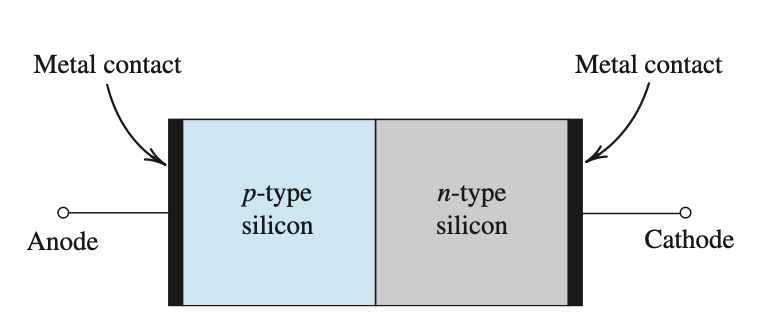
\includegraphics{figs/ch03/pn_junction.png}
    \caption{Simplified physical structure of the PN junction}
\end{figure}

\section{Diffusion Current}
Although it doesn't show it in the diagram, there minority holes generated by thermal ionization in the $n$-type material and there are minority electrons generated in the $p$-type material. Due to concentration difference of holes in the $p$ region and the $n$ region, holes diffuse across the junction from the $p$ side to the $n$ side. This results in \textbf{diffusion current, $I_D$}, whose direction is from the $p$ to $n$ side.

So current Damanic is wondering right now "if this stuff is diffusing then won't this entire block be the same mush at the end." Here we introduce the depletion region. Holes that diffuse across the junction into the $n$ region recombine with majority electrons there. A charge is said to be \textbf{uncovered} when some of the bound positive charge is no longer neutralized by free electrons. This introduces the idea that at a region close to the junction, it is depleted of free electrons and contains unbound positive charge for the $n$ region.

\begin{figure}[H]
    \centering
    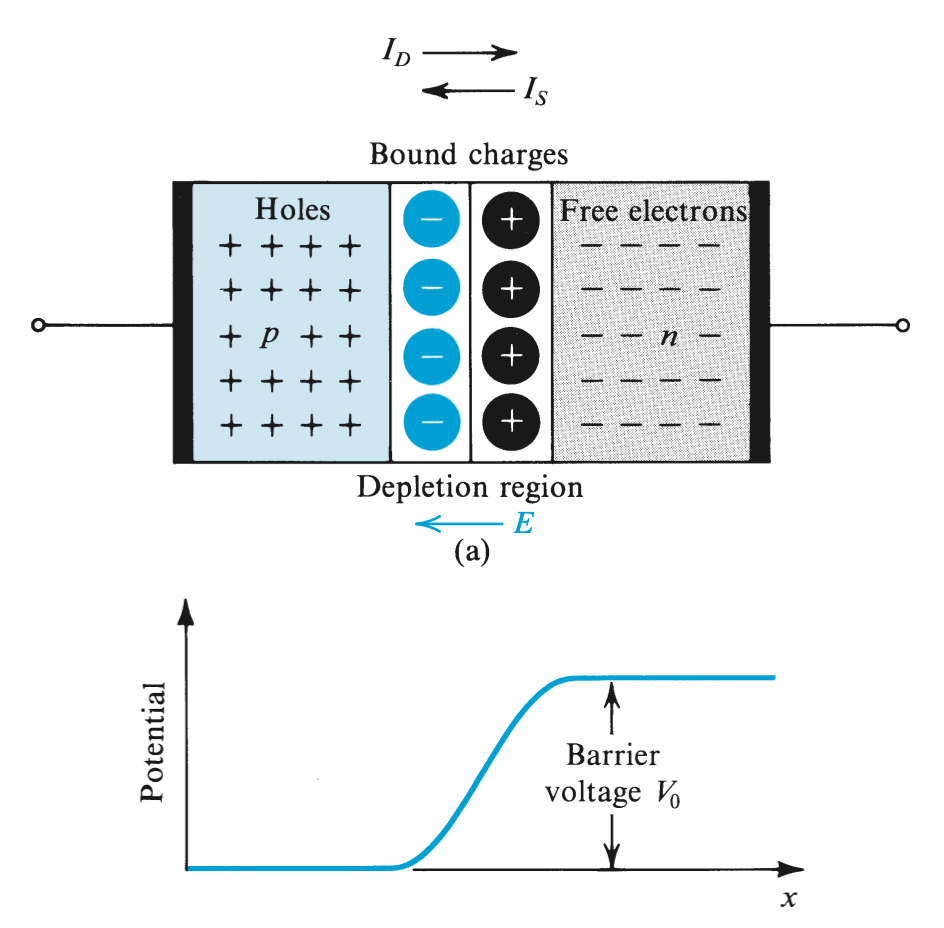
\includegraphics[scale=0.5]{figs/ch03/uncovered_region.png}
    \caption{Top image shows PN-junction with bound charges and bottom image is potential along an axis perpendicular to the junction}
    \label{fig:barrier-voltage1}
\end{figure}

The left side of the PN junction ($p$ region) will be negatively charged while the right side ($n$ region) will be positively charged. To sum it up, this is because at some point, electrons that diffuse across the junction into the $p$ region will recombine with holes, and those holes will disappear leaving uncovered bound negative charge. Vice versa for holes diffusing into the $n$ region. 

From the figure above we see that the $n$ region will be positively charged and the $p$ side if negatively charged. This is the \textbf{depletion region}, or the \textbf{space-charge region} or \textbf{depletion layer}. There are no \textit{mobile} charge carriers present here. Charges on both sides of the depletion region results in an electric field $E$. Here we introduce the idea that a larger barrier voltage results in a small number of carriers that can overcome this barrier. This leads to a decrease in magnitude of diffusion current since it is more difficult for holes to diffuse into the $n$ region and electrons to diffuse into the $p$ region. Referring again to figure \ref{fig:barrier-voltage1}, we see that $V_0$ is the barrier voltage. Therefore the diffusion current $I_D$ has a strong relationship with $V_0$, the voltage drop across the depletion region.

\section{Drift Current and Equilibrium}
Recall that drift current is caused by electric fields and $I_S$ is independent of the value of the depletion-layer voltage $V_0$. Under open-circuit conditions, there is no external current, so 
    \[I_D = I_S\]
This condition is maintained by $V_0$.
\begin{Analysis}{$I_S$ and $I_D$ at Equilibrium}{}
    \begin{gline}
        \item $V_O$: barrier voltage
        \item $I_S$: drift current whose direction is from the $n$ side to the $p$ side of the junction
        \item $I_D$: diffusion current whose direction is from the $p$ side to the $n$ side of the junction
    \end{gline}
    \begin{enumerate}
        \item \textbf{$I_D > I_S$}: more bound charge is uncovered on both sides $\rightarrow$ the depletion layer widens (vertically)$\rightarrow$ $V_0$ increases $\rightarrow$ $I_D$ decreases until $I_D = I_S$ (equilibrium)
        \item \textbf{$I_D < I_S$}: uncovered charge decreases $\rightarrow$ depletion layer narrows (vertically) $\rightarrow$ $V_0$ decreases $\rightarrow$ $I_D$ increases until $I_D = I_S$ (equilibrium)
    \end{enumerate}
\end{Analysis}

Under the zero bias equilibrium condition (no external voltage is applied to the PN junction), does the diffusion and drift current "cancel" out here, meaning that current density is zero. Their individual components are also equal here, i.e. hole/electron drift current is equal to hole/electron diffusion current, respectively.
    \[J_n = 0 = qn_0 \mu_n E_0 + q D_n \frac{dn_0}{dx}\]

$V_0$ has been referred to so far as barrier voltage boltage, but it's also called \textbf{junction built-in voltage}.
    \[\phi_{bi} = V_{th} \ln \left(\frac{N_A N_D}{n_i^2}\right) = \frac{kT}{q} \ln \left(\frac{N_A N_D}{n_i^2}\right)\]
Remember here that $V_th$ is thermal voltage which is $\approx$ 26 mV at room temperature. $\phi_{bi}$ is typically 0.6 V to 0.9V for room temperature silicon. In the EE105 reader, $\phi_{bi}$ and $V_{th}$ has the same meaning as $V_0$ and $V_T$, respectively, in the \textit{Microelectronic Circuits} textbook. I'm writing down the EE105 reader notation here for clarity.

\begin{figure}[H]
    \centering
    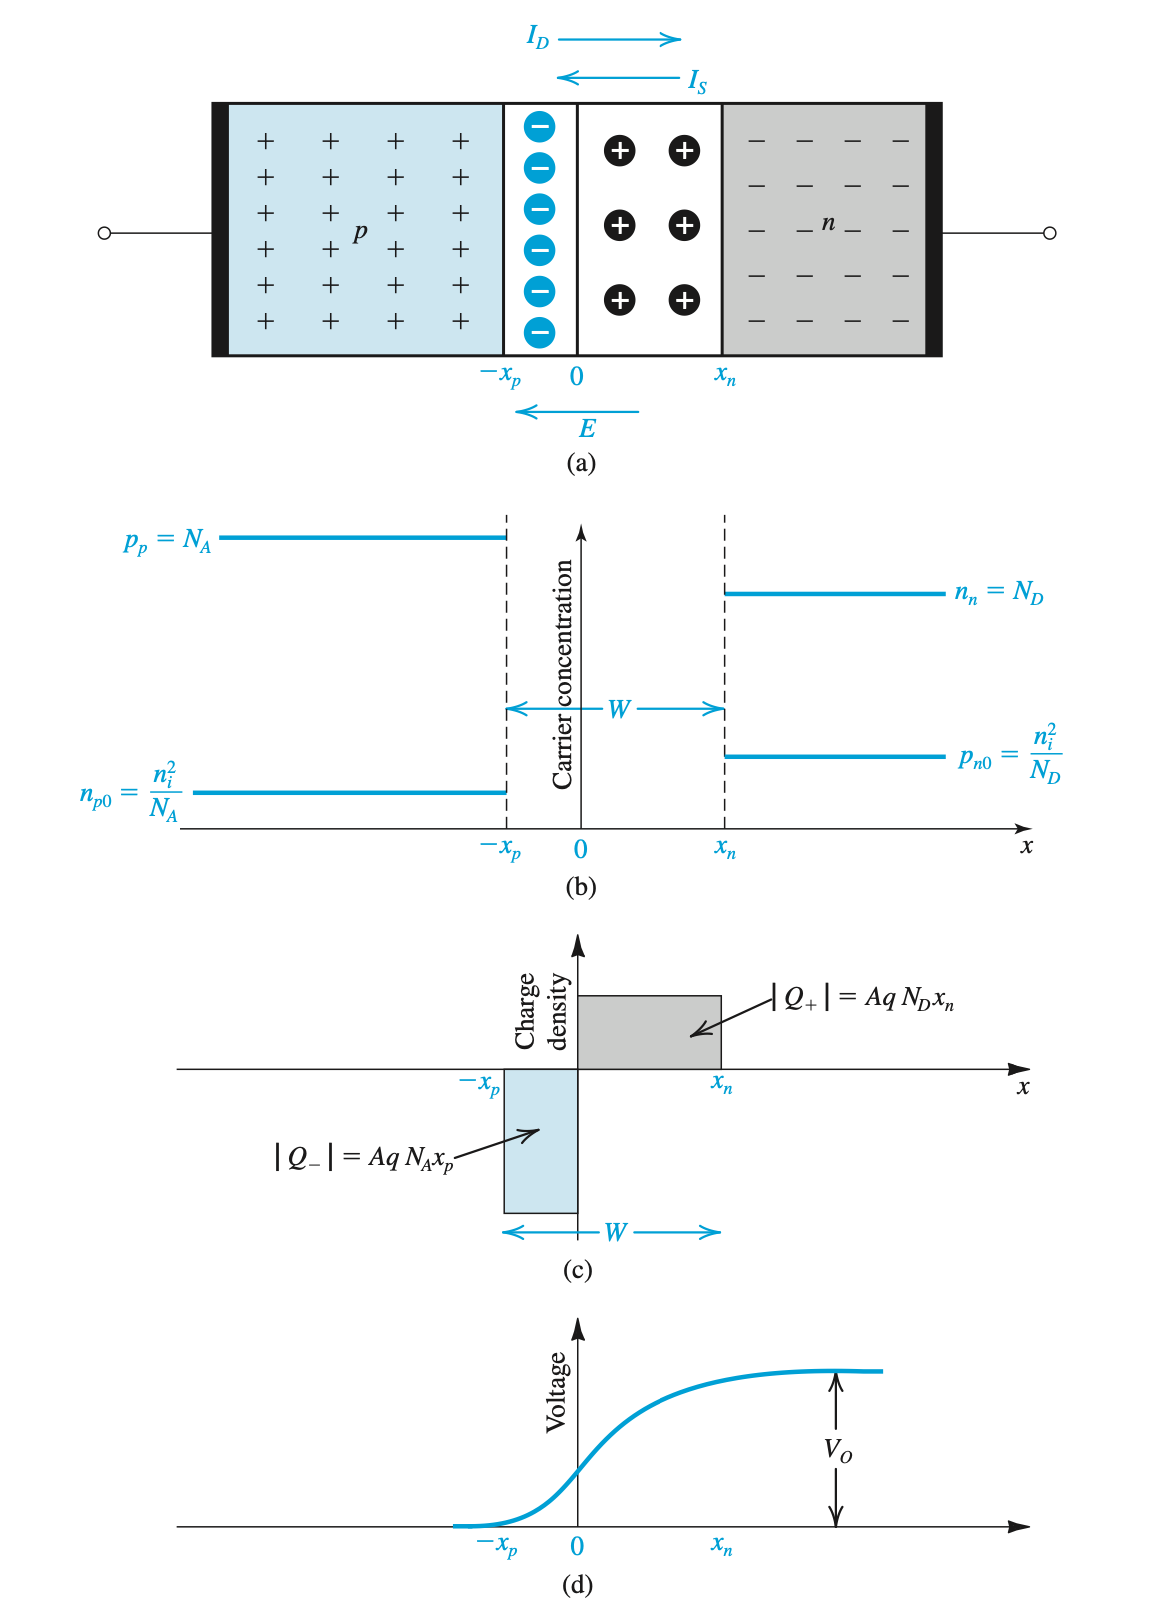
\includegraphics[scale=0.6]{figs/ch03/3_graph.png}
    \caption{Graphs of (a) a PN junction (b) carrier concentrations (c) charge density (d) built in voltage $V_0$}
    \label{fig:3figs}
\end{figure}
How we got from each graph.
\begin{itemize}
    \item 
\end{itemize}

\begin{figure}[H]
    \centering
    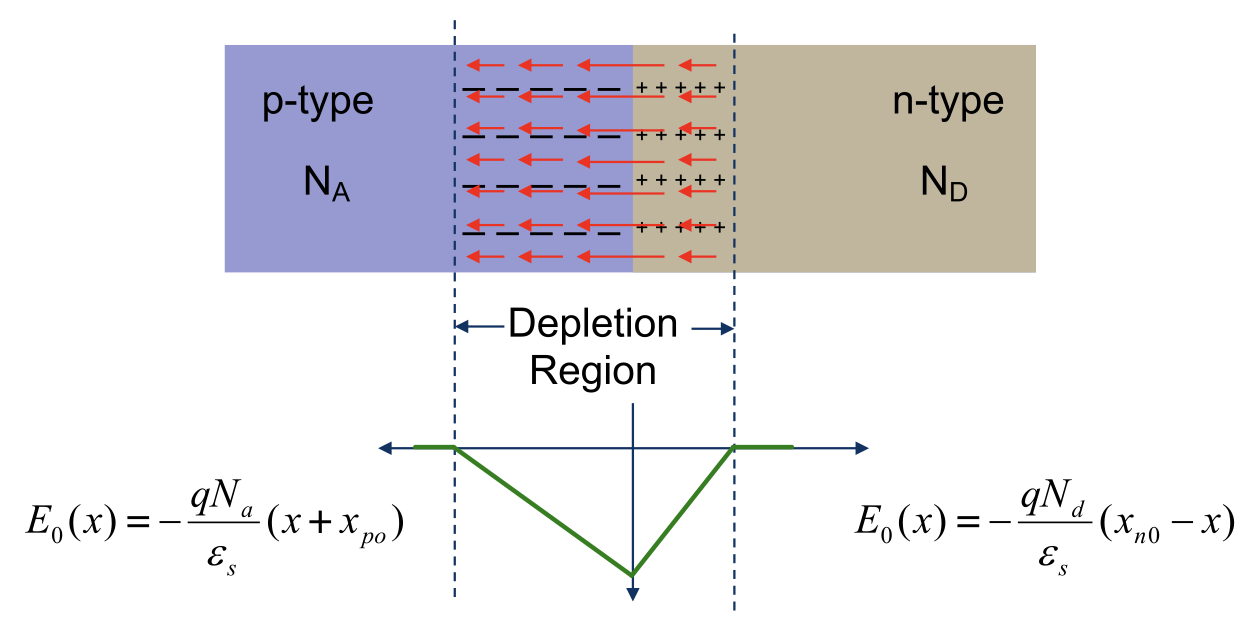
\includegraphics[scale=0.5]{figs/ch03/concentration_reader.png}
    \caption{Graph of electric field of PN junction}
    \label{fig:electric_fields_pn}
\end{figure}
Here in figure \ref{fig:electric_fields_pn}, the electric fields in the depletion region are negative because positive charges are on the right and the negative charges are on the left, assuming zero fields in neutral $P$-region and $N$-regions. Key takeaways:
\begin{pline}
    \item Width of the depletion region is not symmetric
    \item The negative peak of the electric field always occurs at the junction
\end{pline}

\section{Reverse Bias}

\section{Forward Bias}

\section{PN Junction with External Voltage Applied}
The above section was discussing the PN junction at equilibrium.

\section{Practice Problems}
\begin{enumerate}
    \item Show that 
        \[V_0 = \frac12 (\frac{q}{\epsilon_s})(\frac{N_A N_D}{N_A + N_D}) W^2\]
    % \begin{Ans}
    %     We know that $\phi_{bi} = V_{th} \ln \left(\frac{N_A N_D}{n_i^2}\right) = \frac{kT}{q} \ln \left(\frac{N_A N_D}{n_i^2}\right)$
    % \end{Ans}
    \item Show that for a PN junction in which the $p$ side is much more heavily dped than the $n$ side (i.e. $N_A \gg N_D$) referred to as a $p^+ n$ diode. The following can be written as follows:
        \begin{align*}
            W &\simeq \sqrt{\frac{2 \epsilon_s}{q N_D}V_0}, ~~~~~ x_n \simeq W, ~~~~~ x_p \simeq \frac{W}{N_A / N_D} \\
            Q_j &\simeq A q N_D W, ~~~~~ Q_j \simeq A \sqrt{2 \epsilon_s q N_D V_0}
        \end{align*}
    
    \item 
\end{enumerate}

\section{Sources}
\begin{itemize}
    \item Sedra, Adel S., et al. Microelectronic Circuits. Oxford University Press, 2021: Specifically screenshots of the graphs I need to redo this when I learn how to use graphing/tikzpicture better in LaTex
    \item \href{https://file.notion.so/f/f/048d6522-202b-48d4-b5d9-bc005bd602e2/214bf1f0-292f-48d6-9016-737d9f5da155/ee105_reader_v3.pdf?id=237a4300-3dbe-47d1-888b-ffae90d8352b&table=block&spaceId=048d6522-202b-48d4-b5d9-bc005bd602e2&expirationTimestamp=1714435200000&signature=yx-H1qvZJIodPfazOpwXX0Ce2mWMG8skOHl45xoPxus&downloadName=ee105_reader_v3.pdf}{EE105 Reader}
\end{itemize}